\chapter{Mehrdimensionale Integralrechnung}
\section{Doppelintegrale}
Allgemeine Form:
\[ V = \iint\limits_A f(x,y)\di A \]
Über Rechteck-Gebiete ($a\leq x\leq b, c\leq y\leq d$):
\[ V=\iint\limits_{A}f(x,y)\di A = \int_{c}^{d}\int_{a}^{b}f(x,y)\di x\di y \]
Begrenzt durch $y=g_u(x)$ und $y=g_o(x)$:
\[ V = \int_{a}^{b} \int_{g_u(x)}^{g_o(x)} f(x,y)\di y\di x \]
Begrenzt durch $x=h_l(y)$ und $x=h_r(y)$:
\[ V = \int_{c}^{d} \int_{h_l(y)}^{h_r(y)} f(x,y)\di x\di y \]

\subsection{Polarkoordinaten}
\[ V = \iint\limits_A f(r,\theta)\di A = \int_{\alpha}^{\beta}\int_{g_1(\theta)}^{g_2(\theta)}
	f(r,\theta)r\di r \di \theta \]
mit
\[ x = r\cdot\cos\theta \qquad y = r\cdot\sin\theta \]
	
\subsection{Oberfläche}
\[ S = \iint\limits_{R} \sqrt{(f_x)^2+(f_y)^2+1}\di A \]

\subsection{Variablentransformation}
Anstelle der ($x,y$)-Variablen werden ($u,v$)-Variablen verwendet:
\[\begin{aligned} x &= x(u,v) \\ y &= y(u,v) \end{aligned}\]
Das Flächenelement $\di A = \di x\di y$ wird transformiert:
\[ \di x \di y= |D|\di u \di v \]
Die Determinante der \textit{Jacobischen Matrix} ist gegeben durch:
\[ D = \begin{vmatrix} \pdifrac{x}{u} & \pdifrac{x}{v} \\
	\pdifrac{y}{u} & \pdifrac{y}{v} \end{vmatrix} \]
Das neue Integral ist
\[ \iint\limits_R f(x,y)\di x\di y = \iint\limits_R \tilde{f}(u,v)|D|\di u\di v \]


\section{Dreifachintegrale}
Masse eines Körpers $\Omega\subset\mathds{R}^3$:
\[ m = \iiint\limits_{\Omega}\rho(x,y,z)\di V \]
Über Rechteckgebiet ($a\leq x\leq b, c\leq y\leq d,e\leq z\leq f$):
\[ \iiint\limits_\Omega f(x,y,z)\di V = 
	\int_{e}^{f}\int_{c}^{d}\int_{a}^{b}f(x,y,z)\di x\di y\di z  \]

\subsection{Zylinderkoordinaten}
\[ V = \iiint\limits_G f(x,y,z)\di V
	=\iiint\limits_{\tilde{G}} \tilde{f}(r,\theta,z)r\di r\di\theta\di z \]
Variablen werden ersetzt mit:
\[\begin{aligned}
	x &= r\cdot\cos\theta\\
	y &= r\cdot\sin\theta\\
	z &= z \end{aligned}\]

\subsection{Kugelkoordinaten}
\begin{center}
	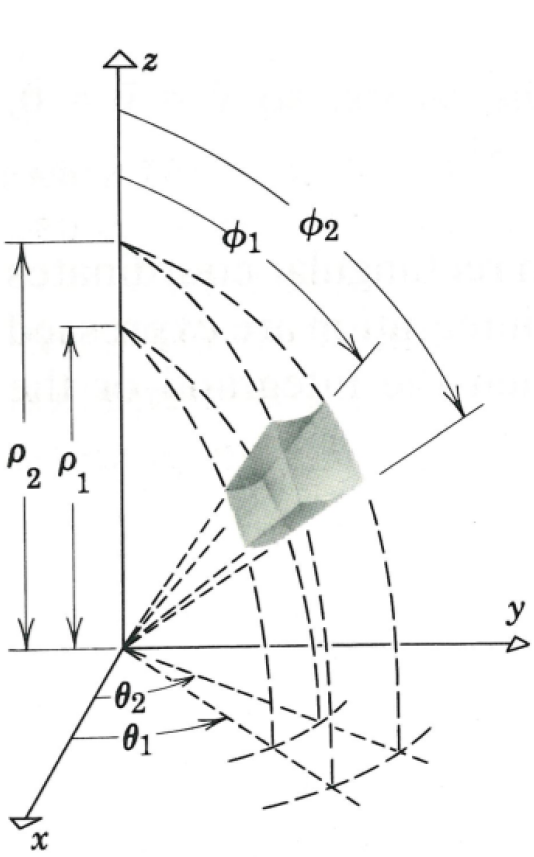
\includegraphics[width=.25\textwidth]{../fig/kugelkoordinaten.png}
\end{center}
\[ V = \iiint\limits_G f(x,y,z)\di V
	=\iiint\limits_{\tilde{G}} \tilde{f}(r,\phi,\theta)r^2\sin\phi\di r\di\phi\di\theta \]
Variablen werden ersetzt mit:
\[\begin{aligned}
	x &= r\cdot\sin\phi\cos\theta\\
	y &= r\cdot\sin\phi\sin\theta\\
	z &= r\cdot\cos\phi \end{aligned}\]
	
\section{Schwerpunkte}
Der \textit{Schwerpunkt $\vec{r}_S$} eines Körpers $\Omega$ mit der Dichte
$\rho=\rho(\vec{r})=\rho(x,y,z)$ ist gegeben durch:
\[ \vec{r}_S = \frac{1}{m}\iiint\limits_\Omega \vec{r}\rho(\vec{r})\di V \]
wobei die Masse $m$ geben ist durch:
\[ m = \iiint\limits_{\Omega}\rho(\vec{r})\di V \]
~\\
Oder die einzelnen Komponenten:
\[\begin{aligned}
	x_S &= \frac{1}{m}\iiint\limits_\Omega x\rho(\vec{r}) \di V\\
	y_S &= \frac{1}{m}\iiint\limits_\Omega y\rho(\vec{r}) \di V\\
	z_S &= \frac{1}{m}\iiint\limits_\Omega z\rho(\vec{r}) \di V\\
\end{aligned}\]

\section{Trägheitsmomente}
Trägheitsmoment ($z$-Achse als Bezugsachse):
\[ I_z = \rho\cdot\iiint\limits_\Omega r^2\di V=\rho\cdot\iiint\limits_\Omega (x^2+y^2)\di V \]
Trägheitstensor \textbf{I} mit Zentrum $\vec{r}_s$:
\[ \textbf{I}_{ik} = \iiint\limits_\Omega(r^2\delta_{ik}-r_ir_k)\di m
	= \rho\cdot\iiint\limits_\Omega(r^2\delta_{ik}-r_ir_k)\di V \]
mit $\delta_{ik}$ als Kronecker-Delta:
\[ \delta_{ik} = \left\lbrace \begin{matrix}
	1, & \text{ falls }i=k \\ 0, & \text{ falls }i\neq k \end{matrix} \right. \]
